\documentclass[]{article}
\usepackage{lmodern}
\usepackage{amssymb,amsmath}
\usepackage{ifxetex,ifluatex}
\usepackage{fixltx2e} % provides \textsubscript
\ifnum 0\ifxetex 1\fi\ifluatex 1\fi=0 % if pdftex
  \usepackage[T1]{fontenc}
  \usepackage[utf8]{inputenc}
\else % if luatex or xelatex
  \ifxetex
    \usepackage{mathspec}
  \else
    \usepackage{fontspec}
  \fi
  \defaultfontfeatures{Ligatures=TeX,Scale=MatchLowercase}
\fi
% use upquote if available, for straight quotes in verbatim environments
\IfFileExists{upquote.sty}{\usepackage{upquote}}{}
% use microtype if available
\IfFileExists{microtype.sty}{%
\usepackage{microtype}
\UseMicrotypeSet[protrusion]{basicmath} % disable protrusion for tt fonts
}{}
\usepackage[margin=1in]{geometry}
\usepackage{hyperref}
\hypersetup{unicode=true,
            pdftitle={Energetic Consequences of Sonar Exposure},
            pdfborder={0 0 0},
            breaklinks=true}
\urlstyle{same}  % don't use monospace font for urls
\usepackage{longtable,booktabs}
\usepackage{graphicx,grffile}
\makeatletter
\def\maxwidth{\ifdim\Gin@nat@width>\linewidth\linewidth\else\Gin@nat@width\fi}
\def\maxheight{\ifdim\Gin@nat@height>\textheight\textheight\else\Gin@nat@height\fi}
\makeatother
% Scale images if necessary, so that they will not overflow the page
% margins by default, and it is still possible to overwrite the defaults
% using explicit options in \includegraphics[width, height, ...]{}
\setkeys{Gin}{width=\maxwidth,height=\maxheight,keepaspectratio}
\IfFileExists{parskip.sty}{%
\usepackage{parskip}
}{% else
\setlength{\parindent}{0pt}
\setlength{\parskip}{6pt plus 2pt minus 1pt}
}
\setlength{\emergencystretch}{3em}  % prevent overfull lines
\providecommand{\tightlist}{%
  \setlength{\itemsep}{0pt}\setlength{\parskip}{0pt}}
\setcounter{secnumdepth}{0}
% Redefines (sub)paragraphs to behave more like sections
\ifx\paragraph\undefined\else
\let\oldparagraph\paragraph
\renewcommand{\paragraph}[1]{\oldparagraph{#1}\mbox{}}
\fi
\ifx\subparagraph\undefined\else
\let\oldsubparagraph\subparagraph
\renewcommand{\subparagraph}[1]{\oldsubparagraph{#1}\mbox{}}
\fi

%%% Use protect on footnotes to avoid problems with footnotes in titles
\let\rmarkdownfootnote\footnote%
\def\footnote{\protect\rmarkdownfootnote}

%%% Change title format to be more compact
\usepackage{titling}

% Create subtitle command for use in maketitle
\newcommand{\subtitle}[1]{
  \posttitle{
    \begin{center}\large#1\end{center}
    }
}

\setlength{\droptitle}{-2em}

  \title{Energetic Consequences of Sonar Exposure}
    \pretitle{\vspace{\droptitle}\centering\huge}
  \posttitle{\par}
    \author{}
    \preauthor{}\postauthor{}
    \date{}
    \predate{}\postdate{}
  

\begin{document}
\maketitle

What are the energetic consequences for cetaceans when exposed to sonar?
The following model makes a first order approximation by estimating (1)
the energy intake lost to foraging cessation and (2) the additional
energy expenditure from increased swim speeds. We considered these two
factors in four potential scenarios:

\begin{enumerate}
\def\labelenumi{\arabic{enumi}.}
\tightlist
\item
  No response
\item
  Cessation of foraging without flight
\item
  Cessation of foraging with flight
\item
  Extreme response
\end{enumerate}

The model was paramterized using data and models from other sources (see
table below). We used functional responses (e.g.~mean flight distance)
from the literature. The energy cost of lost feeding opportunities were
estimated with the scaling relationship between body size and feeding
rate in Jeremy's scaling paper. The energy cost of increased swim speeds
during flight were estimated using models from Williams et al. 2017.

\subsection{Literature}\label{literature}

\begin{longtable}[]{@{}llrl@{}}
\toprule
Reference & Species & N\_tags & Notes\tabularnewline
\midrule
\endhead
Tyack et al. 2011 & Mesoplodon densirostris & 1 & Only 1 tag, but other
data from sonar array\tabularnewline
DeRuiter et al. 2017 & Balaenoptera musculus & 37 & How did the
transition probability from deep feeding to other states change in
CEEs?\tabularnewline
DeRuiter et al. 2013 & Ziphius cavirostris & 2 & Reduced time foraging
in response to proximal sonar, but not distant\tabularnewline
Friedlaender et al. 2016 & Balaenoptera musculus & 9 & Includes prey
data\tabularnewline
Goldbogen et al. 2013 & Balaenoptera musculus & 17 & Basis for
Friedlaender et al. 2016 and DeRuiter et al. 2017\tabularnewline
Kvadsheim et al. 2017 & Balaenoptera acutorostrata & 4 & SoCal + Norway.
1 CEE + 1 control in each location\tabularnewline
Southall et al. 2019 & Ziphius cavirostris & 0 & Prey distribution in
SoCal sonar array\tabularnewline
\bottomrule
\end{longtable}

\subsection{Functional responses}\label{functional-responses}

\emph{Fill me in}

\subsection{Energetic parameters}\label{energetic-parameters}

Energy acquired from prey scales sublinearly among odontocetes
{[}E\textsubscript{p}=0.12M\textsubscript{c}\textsuperscript{0.81}{]}
but superlinearly among mysticetes
{[}E\textsubscript{p}=5.83M\textsubscript{c}\textsuperscript{2.37}{]}.
\emph{Note: Jeremy's paper has a negative coefficient for mysticete
E\textsubscript{p} scaling (v8.3:115) but I think that's a mistake.}

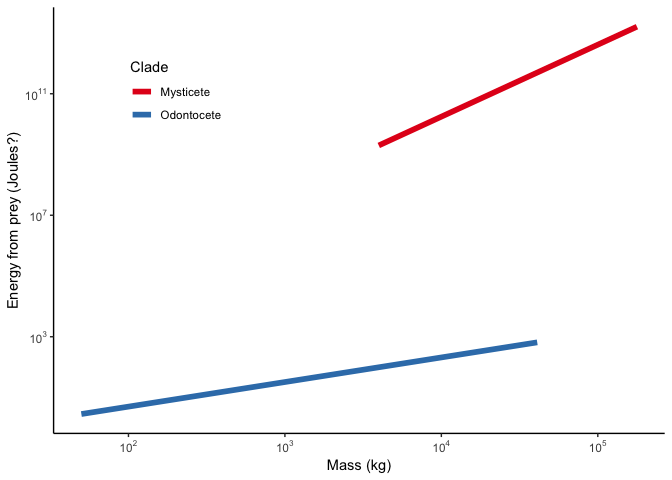
\includegraphics{sonar-response_files/figure-latex/Ep_scaling-1.pdf}

\emph{If I understand correctly, E\textsubscript{p} is energy per
feeding event, so to get energy intake per unit time we also need the
scaling equation for feeding rate. Figure 2 in Jeremy's paper has
{[}feeding events / dive{]} \textasciitilde{} {[}dive time - TADL{]}.
Can we get feeding rates from something like that?}


\end{document}
